\documentclass[a4paper, 11pt]{article}
\usepackage{graphicx}
\usepackage{amsmath}
\usepackage[pdftex]{hyperref}

% Lengths and indenting
\setlength{\textwidth}{16.5cm}
\setlength{\marginparwidth}{1.5cm}
\setlength{\parindent}{0cm}
\setlength{\parskip}{0.15cm}
\setlength{\textheight}{22cm}
\setlength{\oddsidemargin}{0cm}
\setlength{\evensidemargin}{\oddsidemargin}
\setlength{\topmargin}{0cm}
\setlength{\headheight}{0cm}
\setlength{\headsep}{0cm}

\renewcommand{\familydefault}{\sfdefault}

\title{Data Mining: Learning from Large Data Sets - Fall Semester 2015}
\author{Lukasstr@ethz.ch\\ buehlmic@student.ethz.ch\\ habichta@student.ethz.ch\\}
\date{\today}

\begin{document}
\maketitle

\section*{Approximate near-duplicate search using Locality Sensitive Hashing} 


The implementation follows a \textit{Min-hashing} approach as a locality sensitive hashing scheme. The main bulk of the implementation focuses on creating a \textit{signature matrix} $M$.  In each row, $M$ contains the minimum indices of non-zero column values, found in the row-wise permuted \textit{shingle matrix} $S$. $S$ is permuted several times by defining a linear hash function $\pi(r)$, which is defined as follows.
$$ \pi_{i}(r) =  a_{i}r + b \bmod n$$
The function describes the $i$-th permutation of a row $r$ of the matrix $S$. The exact permutation of all rows is determined by the randomly generated values $a_{i}$ and $b$. In order to reduce the number of hash collisions, $n$ signifies a  prime number. The function $h_{\pi_{i}}(C)$ is then applied to each permutation of $S$.
$$h_{\pi_{i}}(C)  = \min_{r:C(r)=1} \pi_{i}(r)$$
Applied to each input document (video), this creates the $i$-th row of $M$. According to the law of large numbers, the (row-wise) similarity of the columns in M will converge to the \textit{Jaccard similarity}. Increasing the number of permutations (hash functions) decreases the rate of false negatives. However, it also increases the number of false positives. Therefore, this implementation uses a composition of r-way AND and b-way OR hash functions. $M$ is partitioned into $b$ bands with $r$ rows each. Each band $j$ hashes its columns to a specific value, called a $bucket$. For each band, we apply $h(s)$

$$h(s) = \displaystyle\sum_{i=1}^{r} a_{i}s_{i} + b \bmod n $$

$s$ is a vector of size r, containing the values of a column within a band. The other parameters have the same meaning as described above. However, different values are chosen. Videos, whose bands appear in the same bucket at least once are then further investigated. Their shingles are compared to derive the Jaccard similarity. If the similarity is at least 90\%, their identification numbers are outputted.

The implementation uses the \textit{MapReduce} paradigm to exploit the inherent parallelism found in the approach described above. \newline The \textit{Mapper} processes are responsible for creating $M$ and hashing the the bands into their respective buckets. At the beginning, they define the number of hash functions which can be derived by the multiplication of the \texttt{band\_size} ($r$) and the \texttt{num\_bands} ($b$). In this implementation, $r$ amounts to 25 and $b$ is 39. Consequently, the number of hash functions is 975 for the signature matrix plus 39 for the hash bands. Hence we have 975 + 39 = 1014 hash functions in total. This performs quite well and gives us only a very small amount of False-Negatives (see Figure \ref{perfPlot}). (Remark: In our latest version we fixed \texttt{band\_size} = 16 and \texttt{num\_bands} = 60. With that we got a score of 1.0.)
\begin{figure}
	\begin{center}
		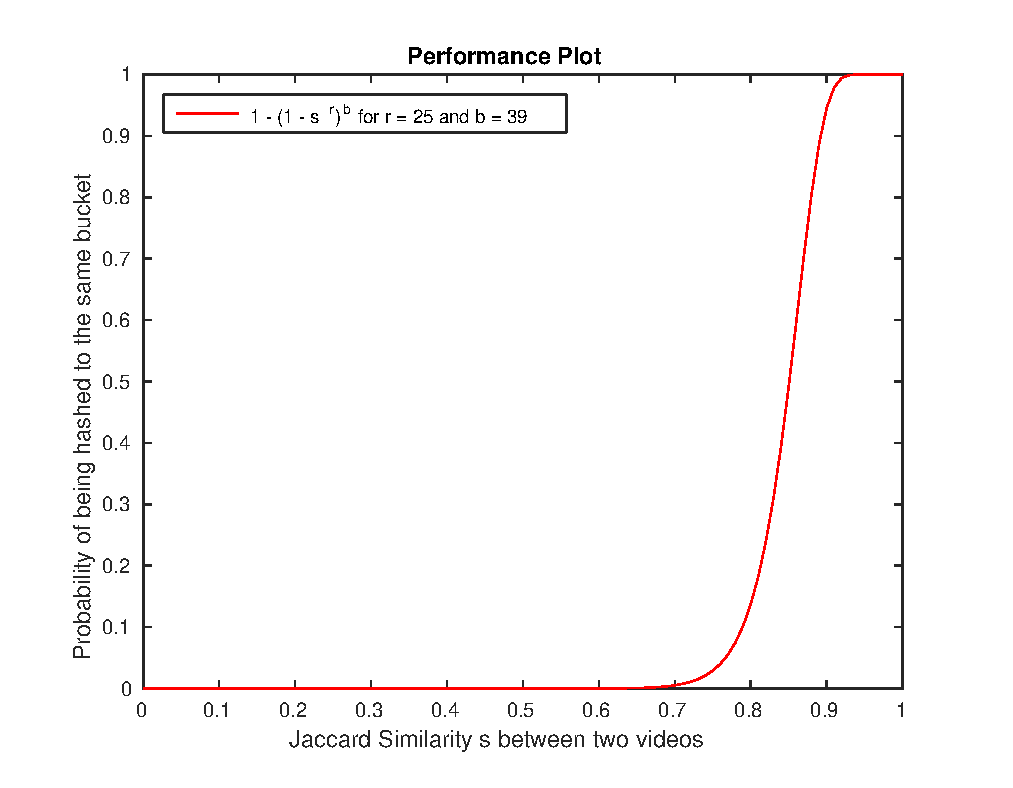
\includegraphics[scale=0.4]{performance}
		\caption{Plots the probability that two videos are being hashed to the same bucket against the Jaccard Similarity of the two videos.}
		\label{perfPlot}
	\end{center}
\end{figure}

Furthermore, the \texttt{numpy} library is used to generate random values for the calculations outlined above. The Mapper receives the \texttt{video\_id} and the corresponding  \texttt{shingles}. It then constructs one column of the signature matrix of that video by calling \texttt{construct\_column\_from\_shingles()}. It uses a matrix initialized with a value larger than the largest possible shingle value. Since the shingle value concurs with the non-zero indices of $S$ (one column per video), finding the minimum shingle value after permuting the rows of the column is equivalent to finding the smallest non-zero index. This is done iteratively. The function loops over each shingle and row of $M$ (this is the same as iterating over each hash function), does a linear hash, and finds the minimum for each row. This yields a full column of $M$. \newline 
Afterwards, it defines the bands with \texttt{hash\_bands()}. It calculates the buckets in which each band of the column is mapped and returns a map \texttt{hash\_values} to save this mapping. The Mapper then returns  strings of the form ``\texttt{\%s \%s\textbackslash t\%s \%s}''. The first value is the \texttt{band\_number} and the second the \texttt{hash\_values[band\_number]}. The letter signifies the bucket number in which the respective band was hashed. Both values form the key that is later used by the reducer. The remaining values are the \texttt{video\_id} and the sorted \texttt{shingles}.

The \texttt{Reducer} processes receive the Mapper's outputs in a sorted manner (sorted by the key).  The Reducer first parses the input and checks if a specific key was seen before. If this is the case, then a possible duplicate is detected (the same bands of different videos are hashed into the same bucket). The possible duplicates are saved in a set. As soon as a new key appears, this set is evaluated by the \texttt{print\_duplicates()} function. This function compares all the possible duplicates with each other by calculating the Jaccard similarity of all their shingles. if it is larger or equal to 90\%, it prints both \texttt{video\_ids} in ascending order.
\newpage

\section*{Large Scale Image Classification} 

In order to tackle the large scale image classification problem for two different kinds of images, we employed a multitude of different techniques which all revolve around stochastic gradient descent. Our focus lied on the mapper function, while the reducer simply averages all the incoming coefficients that define the seperating hyperplane. 

Our first approach was to implement a simple support vector machine by employing the simple algorithm discussed in the lecture. We attempted to solve the online convex programming problem by iteratively calculating a new coefficient vector $w_{t+1}$ from a previous $w_{t}$, using the following algorithm
$$w_{t+1} = w_{t} - \eta_{t}\nabla f_{t}(w_{t})  $$
whereas $\eta_{t}$ is the step size and $f_{t}$ the convex loss function. We used the \textit{hinge loss} to generate a support vector machine. Apart from adjusting $w_{t}$ by subtracting the (sub-) gradient, we also projected it to a sphere of radius $1/\sqrt{\lambda}$. $\lambda$ is the regularization parameter of our convex optimization problem.\\
We used a binary search approach to tune our regularization parameter. However, the results were not satisfactory (evaluating to a score of around 0.5). We improved our accuracy by scaling the image feature vectors by using either the \textit{min-max scaler} or the \textit{scaler} functions provided by the \textit{scikit-learn} library. This improved our score dramatically to over 0.7. Still, we fell short to the hard baseline and we devised different approaches. \\
A slight improvent could be registered by implementing a non-batch version of the \textit{Pegasos} algorithm. This was a natural choice, because only few changes to our original algorithm were necessary. We changed $f_{t}$ to render it strongly convex by adapting the update step to 
$$ w_{t+1} \leftarrow (1-\eta_{t}\lambda)w_{t} + \eta_{t}y_{t}x_{t} $$
The hope was to exploit faster convergence due to strongly convex loss functions. However, the performance was underwhelming. Therefore, we decided to abandon manual implementation of stochastic gradient descent and employ methods provided by \textit{scikit-learn}. 

The obvious choice fell upon the \texttt{SGDClassifier} function. Since the problem had to be solved in an online setting, we used the \texttt{partial\_fit} function to iteratively update our coefficient vector, which we outputted by reading the \texttt{\_coef} field. Apart from simply using the \texttt{SGDClassifier}, we also attempted to implement \textit{Random Fourier Features}. However, these appeared to be too costly (computation-wise). After undertaking many different tests with different settings and parameter values (concerning the regularization parameter, averaging and loss functions), we settled on a particular configuration which would maximize our score. Our highest score was almost 0.8 by using a regularization parameter of $1^{-7}$ and averaging over intermediate coefficient vectors (average value of 1000).
\newpage

\section*{Extracting Representative Elements} 
We used a rather simple approach to solve this clustering problem.\\At first, we skipped any computations in the mapper and just forwarded all data points to the reducer, where we then applied the KMeans algorithm. This worked, but gave us pretty poor results, way below the easy baseline.\\\\
It was obvoius that we needed to improve the mapper. In our second approach we used the mapper to calculate a spefic number of cluster centers using the MiniBatch-KMeans-algorithm provided by the sklearn.cluster library. We then forwarded the resulting center points to the reducer. The reducer uses the standard KMeans algorithm form sklearn.cluster with a 100 cluster centers.\\\\
We tried several different numbers for the amount of cluster centers (denoted n) calculated by the mapper:\\For n = 1'000 the program execution takes too long and a time out error occurs.\\ For n = 100 our score barely met the easy baseline. \\ We determined by trial and error that the optimal n is somewhere between 500 and 600. We achieved our best score of 8.64 with n = 550.
\newpage

\section*{Explore-Exploit tradeoffs in Recommender Systems}
To solve this problem, we implemented the LinUCB Algorithm from the lecture. You can find a pseudo code of this algorithm on Slide 16 from Lecture 12 (Contextual bandidts). I will refer to the notation on this slide in the following desccription of our implementation. 

We will now shortly describe our implementation of the functions \emph{set\_articles(dictionary)}, \emph{update(reward)} and \emph{reccomend(time, user\_features, articles)}.
\begin{enumerate}
\item{\emph{set\_articles(dictionary)}:} In this function we receive the available articles as a function argument. The articles are contained in a dictionary, where the key of the items corresponds to the article IDs and the values of the items corresponds to the features of the article IDs. Because the LinUCB Algorithm only uses the user features $z_t$ and not the articles features,we completely ignore the articles features in our implementation. Instead we only initialize the matrices $M_x$ and the vectors $b_x$ of all articles $x$.

\item{\emph{reccomend(time, user\_features, articles)}:} Our implementation loops over all articles $x$ given by the function argument articles and calculates the corresponding upper confidence bound values $UCB_x$. For this we heavily used the python library \emph{numpy}.

Unfortunately our implementation of the \emph{reccomend(.)} function turned out to be too slow. On the server we got a timeout error. By carefully analysing the runtime of our algorithm, we noted that the calculation of the inverse matrix $M_x^{-1}$ was a bottleneck in the running time. We solved the problem by storing $M_x^{-1}$ in the memory and updating it only from time to time in the \emph{update(.)} function. In the \emph{reccomend(.)} function we then just needed to fetch $M_x^{-1}$ and didn't waste time recalculating it for every article.

\item{\emph{update(reward)}:} If the article chosen by our \emph{reccomend(.)} function is the same as the one in the log file, we update our model according to the formulas $M_x \leftarrow M_x + z_tz_t^T$ and $b_x \leftarrow b_x + y_tz_t$ (see again Slide 16 from the Lecture Slides 12). As we already explained in the function \emph{reccomend(.)}, we additionally update the matrix $M_x^{-1}$ from time to time. Every time the number of past updates of an article $x$ is dividable by $10$, we calculate $M_x^{-1}$ from scratch and update it by its new value. If the number of past updates is not dividable by $10$, we don't update $M_x^{-1}$. This allows us to save a lot of calculation time while only losing a small amount of prediction performance.
\end{enumerate}

The procedure explained above, together with the value $0.2$ for the parameter $\alpha$, turned out to give quite good results. We received a score of 0.065799, so we only missed the hard baseline by 0.000026.

\end{document} 
